\documentclass[12pt,compress,aspectratio=169]{beamer}
\usetheme{metropolis}
\setbeamersize{text margin left=.5cm,text margin right=.5cm}
\usepackage[lf]{carlito}
\usepackage{siunitx}
\usepackage{tikz}
\usepackage{mathpazo}
\usepackage{bm}
\usepackage{mathtools}
\usepackage[ISO]{diffcoeff}
\diffdef{}{ op-symbol=\mathsf{d} }
\usepackage{xcolor,colortbl}

\setmonofont{Ubuntu Mono}
\setlength{\parskip}{0pt}
\renewcommand{\baselinestretch}{1}

\sisetup{
  inter-unit-product=\cdot,
  per-mode=symbol
}

\tikzset{
  >=latex
}

%\newcommand{\iii}{\hat{\bm\imath}}
%\newcommand{\jjj}{\hat{\bm\jmath}}
%\newcommand{\kkk}{\hat{\bm k}}


\usetikzlibrary{patterns}

\title{Class 9: Rigid Body Rotational Motion, Part 3}
\subtitle{Advanced Placement Physics C}
\author[TML]{Dr.\ Timothy Leung}
\institute{Olympiads School}
\date{Updated: Summer 2022}

\newcommand{\pic}[2]{
  \includegraphics[width=#1\textwidth]{#2}
}
\newcommand{\eq}[2]{
  \vspace{#1}{\Large
    \begin{displaymath}
      #2
    \end{displaymath}
  }
}
%\newcommand{\iii}{\ensuremath\hat{\bm{\imath}}}
%\newcommand{\jjj}{\ensuremath\hat{\bm{\jmath}}}
%\newcommand{\kkk}{\ensuremath\hat{\bm{k}}}
\newcommand{\iii}{\ensuremath\hat\imath}
\newcommand{\jjj}{\ensuremath\hat\jmath}
\newcommand{\kkk}{\ensuremath\hat k}



\begin{document}

\begin{frame}
  \maketitle
\end{frame}



\section{Review}

\begin{frame}{Curvilinear vs. Rectilinear Motion}
  Kinematic quantities for rectilinear (translational) vs.\ curvilinear
  (circular) motion are related:

  \vspace{-.25in}{\large
    \begin{align*}
      \vec r &\quad\rightarrow\quad \theta \\
      \vec v &\quad\rightarrow\quad \omega \\
      \vec a &\quad\rightarrow\quad \alpha
    \end{align*}
  }

  Dynamics:
  
  \vspace{-.25in}{\large
    \begin{align*}
      m &\quad\rightarrow\quad I\\
      \vec F &\quad\rightarrow\quad\tau\\
      \vec p=m\vec v_\text{cm} &\quad\rightarrow\quad L=I\omega
    \end{align*}
  }
\end{frame}



\begin{frame}{Laws of Motion}
  The laws of motion are also related between translational and rotational
  motion:
  
  \vspace{-.3in}{\large
    \begin{align*}
      \vec F_\text{net}=\diff{\vec p_\text{cm}}t &\quad\rightarrow\quad
      \tau_\text{net}=\diff Lt \\
      \vec F_\text{net}=m \vec a_\text{cm} &\quad\rightarrow\quad
      \tau_\text{net}=I\alpha
    \end{align*}
  }
\end{frame}




\begin{frame}{Mechanical Work}
  Mechanical Work:

  \eq{-.1in}{
    W_t=\int_{\vec x_1}^{\vec x_2}\vec F\cdot\dl\vec x
    \quad\longrightarrow\quad
    W_r=\int_{\theta_1}^{\theta_2}\tau\dl\theta
  }

  Work-energy theorem:

  \eq{-.1in}{
    W_t=\Delta K_t
    \quad\longrightarrow\quad
    W_r=\Delta K_r
  }

  Kinetic Energy:
  
  \eq{-.1in}{
    K_t=\frac12mv_\text{cm}^2
    \quad\longrightarrow\quad
    K_r=\frac12I\omega^2
  }
\end{frame}


\begin{frame}{Kinetic Energy of a Rotating System}
  The total kinetic energy of a rotating system is the sum of its translational
  and rotational kinetic energies at its center of mass:

  \eq{-.1in}{
    \boxed{K=K_t+K_r=\frac12mv_\text{cm}^2+\frac12I_\text{cm}\omega^2}
  }
  
  In this case, $I_\text{cm}$ is calculated at the center of
  mass. For simple problems, we only need to compute rotational kinetic energy
  at the pivot:

  \eq{-.1in}{
    \boxed{K=\frac12I_\text{P}\omega^2}
  }
  
  In this case, the $I_\text{P}$ is calculated at the pivot.
  \textbf{IMPORTANT:} $I_\text{cm}\neq I_\text{P}$
\end{frame}



\section{Rolling on Inclined Surface}

\begin{frame}{Rolling on an Inclined Surface}
  We now re-examine the example problem for a rigid \& smooth sphere of radius
  $R$ rolling down a ramp of angle  $\phi$ without slippage, this time using
  the conservation of energy.

  \vspace{.2in}
  \begin{columns}
    \column{.35\textwidth}
    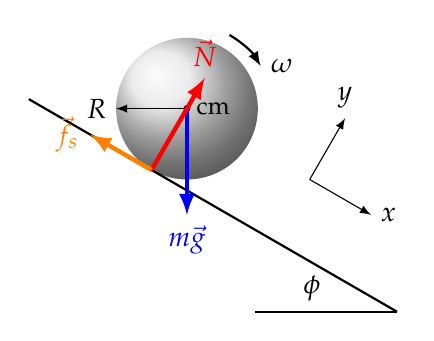
\begin{tikzpicture}[scale=.9]
      \begin{scope}[rotate=-30]
        \shade[ball color=gray!20] circle(1);
        \draw[thick](-2,-1)--(4,-1);
        \draw[->,rotate=30](0,0)--(-1,0) node[left]{$R$};
        \draw[thick,->](0,1.2) arc(90:60:1.2) node[right]{$\omega$};
        \draw[->](2,0)--(3,0) node[right]{$x$};
        \draw[->](2,0)--(2,1) node[above]{$y$};
        \fill circle(.05) node[right]{\small cm};
        \begin{scope}[->,ultra thick]
          \draw[blue,rotate=30](0,0)--(0,-1.5) node[below]{$m\vec g$};
          \draw[red](0,-1)--(0,.5) node[above]{$\vec N$};
          \draw[orange](.0,-1)--(-1,-1) node[left]{$\vec f_s$};
        \end{scope}
        \begin{scope}[rotate around={30:(4,-1)}]
          \draw[thick](4,-1)--(2,-1) node[pos=.6,above]{$\phi$};
        \end{scope}
      \end{scope}
    \end{tikzpicture}

    \column{.65\textwidth}
    Three forces act on the sphere as it rolls down the ramp
    \begin{itemize}
    \item The weight ($mg$) of the sphere acts at the CM
    \item The normal force ($N$) acts at the point of contact
    \item The static friction ($f_s$) act at the point of contact
    \end{itemize}
    Only static friction generates a torque about the CM in the clockwise
    direction
  \end{columns}
\end{frame}



\begin{frame}{Rolling on an Inclined Surface}
  The center of mass of the sphere will translate down the ramp, along the
  $\iii$ direction. The sphere will also rotate in the clockwise direction.

  \vspace{.2in}
  \begin{columns}
    \column{.35\textwidth}
    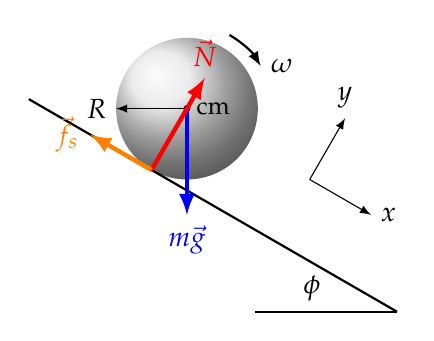
\begin{tikzpicture}[scale=.9]
      \begin{scope}[rotate=-30]
        \shade[ball color=gray!20] circle(1);
        \draw[thick](-2,-1)--(4,-1);
        \draw[->,rotate=30](0,0)--(-1,0) node[left]{$R$};
        \draw[thick,->](0,1.2) arc(90:60:1.2) node[right]{$\omega$};
        \draw[->](2,0)--(3,0) node[right]{$x$};
        \draw[->](2,0)--(2,1) node[above]{$y$};
        \fill circle(.05) node[right]{\small cm};
        \begin{scope}[->,ultra thick]
          \draw[blue,rotate=30](0,0)--(0,-1.5) node[below]{$m\vec g$};
          \draw[red](0,-1)--(0,.5) node[above]{$\vec N$};
          \draw[orange](.0,-1)--(-1,-1) node[left]{$\vec f_s$};
        \end{scope}
        \begin{scope}[rotate around={30:(4,-1)}]
          \draw[thick](4,-1)--(2,-1) node[pos=.6,above]{$\phi$};
        \end{scope}
      \end{scope}
    \end{tikzpicture}

    \column{.65\textwidth}
    The work done by the three forces acting on the sphere:
    \begin{itemize}
    \item Weight ($mg$) does $+$ translational work, but no rotational
      work
    \item Normal force ($N$) does no translational work, and no rotational
      work
    \item Static friction ($f_s$) does $(-)$ translational work, and $(+)$
      rotational work
    \end{itemize}
    Although static friction is non-conservative, the work done stays inside
    the system
  \end{columns}    
\end{frame}



\begin{frame}{Rolling on an Inclined Surface}
  In this case, the system consists of the the sphere and Earth, much like the
  (much simpler) system of a mass sliding down a ramp.

  \vspace{.2in}
  \begin{columns}
    \column{.35\textwidth}
    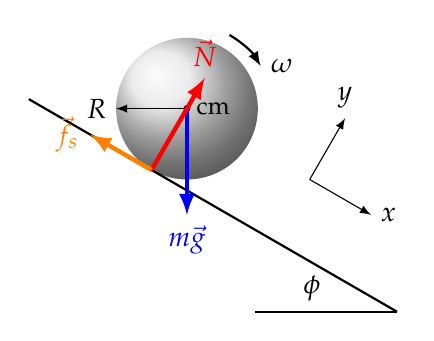
\begin{tikzpicture}[scale=.9]
      \begin{scope}[rotate=-30]
        \shade[ball color=gray!20] circle(1);
        \draw[thick](-2,-1)--(4,-1);
        \draw[->,rotate=30](0,0)--(-1,0) node[left]{$R$};
        \draw[thick,->](0,1.2) arc(90:60:1.2) node[right]{$\omega$};
        \draw[->](2,0)--(3,0) node[right]{$x$};
        \draw[->](2,0)--(2,1) node[above]{$y$};
        \fill circle(.05) node[right]{\small cm};
        \begin{scope}[->,ultra thick]
          \draw[blue,rotate=30](0,0)--(0,-1.5) node[below]{$m\vec g$};
          \draw[red](0,-1)--(0,.5) node[above]{$\vec N$};
          \draw[orange](.0,-1)--(-1,-1) node[left]{$\vec f_s$};
        \end{scope}
        \begin{scope}[rotate around={30:(4,-1)}]
          \draw[thick](4,-1)--(2,-1) node[pos=.6,above]{$\phi$};
        \end{scope}
      \end{scope}
    \end{tikzpicture}

    \column{.65\textwidth}
    The total energy of the system therefore includes:
    \begin{itemize}
    \item The translational kinetic energy of the sphere
    \item The rotational kinetic energy of the sphere
    \item The gravitational kinetic energy stored between the sphere \& Earth
    \end{itemize}
    The system is an isolated system, because there is no external work done
    \begin{itemize}
    \item Although friction is non-conservative, it is \emph{internal} to the
      system
    \end{itemize}
  \end{columns}
\end{frame}



\begin{frame}{Rolling on an Inclined Surface}
  \begin{columns}
    \column{.35\textwidth}
    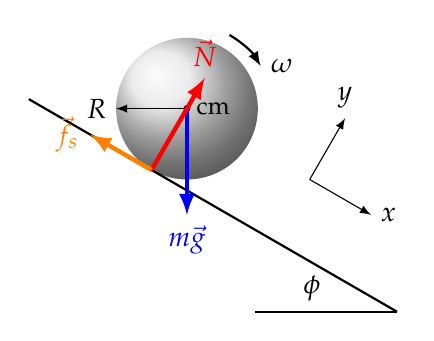
\begin{tikzpicture}[scale=.9]
      \begin{scope}[rotate=-30]
        \shade[ball color=gray!20] circle(1);
        \draw[thick](-2,-1)--(4,-1);
        \draw[->,rotate=30](0,0)--(-1,0) node[left]{$R$};
        \draw[thick,->](0,1.2) arc(90:60:1.2) node[right]{$\omega$};
        \draw[->](2,0)--(3,0) node[right]{$x$};
        \draw[->](2,0)--(2,1) node[above]{$y$};
        \fill circle(.05) node[right]{\small cm};
        \begin{scope}[->,ultra thick]
          \draw[blue,rotate=30](0,0)--(0,-1.5) node[below]{$m\vec g$};
          \draw[red](0,-1)--(0,.5) node[above]{$\vec N$};
          \draw[orange](.0,-1)--(-1,-1) node[left]{$\vec f_s$};
        \end{scope}
        \begin{scope}[rotate around={30:(4,-1)}]
          \draw[thick](4,-1)--(2,-1) node[pos=.6,above]{$\phi$};
        \end{scope}
      \end{scope}
    \end{tikzpicture}

    \column{.65\textwidth}
    As the sphere rolls downward without slipping, the total mechanical
    energy is conserved, i.e.:

    \eq{-.1in}{
      \boxed{
        K_t + K_r + U_g = \text{constant}
      }
    }
    \begin{itemize}
    \item The positive translational work done by gravity converts $U_g$ into
      $K_t$
    \item The work done by static friction converts $K_t$ to $K_r$
    \item All the energy stays inside the system, therefore the system is an
      isolated system
    \end{itemize}
  \end{columns}
\end{frame} 
\end{document}

